\chapter{混合(Blending)}
\begin{flushleft}
考虑图\ref{fig:10-1}。 首先绘制地形,绘制木箱,接着将地形和板条箱像素放在后面的缓冲区上。 然后,使用混合将水面绘制到后缓冲区(back buffer),以便水像素与地形混合,并在后缓冲区上放置像素,使地形和板条箱通过水显示。 在本章中,我们将研究混合技术,这些技术允许我们将当前光栅化的像素(所谓的源像素)与先前光栅化到后缓冲区的像素(所谓的目标像素)混合(组合)。这种技术使我们能够渲染半透明物体,如水和玻璃。\\
\end{flushleft}

\begin{figure}[h]
    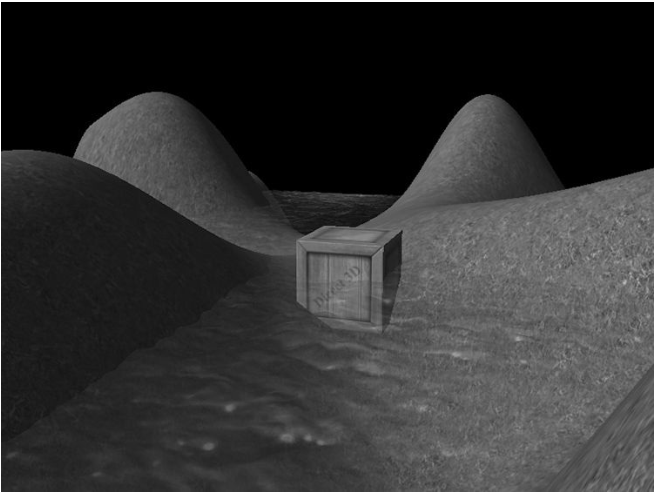
\includegraphics[width=\textwidth]{10-1}
    \centering
    \caption{半透明的水面。}
    \label{fig:10-1}
\end{figure}

\begin{flushleft}
~\\
NOTICE: 为了便于讨论,特别提到后缓冲区作为渲染目标。 但是,稍后将展示可以渲染到“屏幕外”渲染目标。 混合适用于这些渲染目标,目标像素是先前光栅化到这些屏幕外渲染目标的像素值。
~\\
{\large Objectives:}
\begin{itemize}
    \item 1.了解混合的工作原理以及如何将其与Direct3D一起使用。
    \item 2.了解Direct3D支持的不同混合模式。
    \item 3.了解如何使用alpha分量来控制基元(primitive)的透明度。
    \item 4.要了解如何通过使用HLSL clip 函数来阻止像素完全被绘制到后缓冲区。
\end{itemize}
\end{flushleft}

%-------- 10.1 --------
\section{混合公式(The Blending Equation)}
\begin{flushleft}
设$C_{src}$是当前光栅化的第$i$个像素(源像素)的像素着色器的颜色输出,并且设$C_{dst}$是当前在后缓冲器(目标像素)上的第$i$个像素的颜色。 如果没有混合,$C_{src}$将覆盖$C_{dst}$(假设它通过深度/模板测试(depth/stencil test))并成为第$i$个后缓冲区像素的新颜色。 但是通过混合,新颜色$C$将覆盖$C_{dst}$(即,混合颜色$C$将被写入后缓冲器的第$i$个像素)。 Direct3D使用以下混合公式来混合源像素和目标像素颜色:\\
\end{flushleft}

\begin{align*}
C=C_{src}\otimes F_{src}\boxplus C_{dst}\otimes F_{dst}
\end{align*}

\begin{flushleft}
颜色$F_{src}$(源混合因子)和$F_{dst}$(目标混合因子)可以是10.3节中描述的任何值,它们允许以各种方式修改原始源像素和目标像素,获得不同的效果。$\otimes$运算符是5.3.1节中定义的颜色向量的分量乘法; $\boxplus$运算符是10.2节中定义的任何二元运算符。\\

上述混合方程仅适用于颜色的RGB分量。alpha分量实际上由另一个单独公式处理:\\
\end{flushleft}

\begin{align*}
A=A_{src}F_{src}\boxplus A_{dst}F_{dst}
\end{align*}

\begin{flushleft}
等式基本相同,但混合因子和二元运算可能不同。 将RGB与alpha分离的动机很简单,可以独立处理它们,这使混合控制变得更灵活。\\
~\\
NOTICE: 与混合RGB分量相比,混合alpha分量的频率要低得多。 这主要是因为我们不关心后缓冲区alpha值。 如果您有一些需要目标alpha值的算法,则处理后缓冲区alpha值即可。
~\\
\end{flushleft}

%-------- 10.2 --------
\section{混合操作符(Blend Operations)}
\begin{flushleft}
二元运算符$\boxplus$由以下枚举类定义,用于混合公式运算:\\
\end{flushleft}

\begin{lstlisting}[mathescape]
typedef enum D3D12_BLEND_OP
{
    D3D12_BLEND_OP_ADD = 1, $C=C_{src}\otimes F_{src} + C_{dst}\otimes F_{dst}$
    D3D12_BLEND_OP_SUBTRACT = 2, $C=C_{dst}\otimes F_{dst} - C_{src}\otimes F_{src}$
    D3D12_BLEND_OP_REV_SUBTRACT = 3, $C=C_{src}\otimes F_{src} - C_{dst}\otimes F_{dst}$
    D3D12_BLEND_OP_MIN = 4, $C=min(C_{src},C_{dst})$
    D3D12_BLEND_OP_MAX = 5, $C=max(C_{src},C_{dst})$
} D3D12_BLEND_OP;
\end{lstlisting}

\begin{flushleft}
~\\
NOTICE: min/max 操作符忽略混合因子($F$)
~\\

这些运算符也适用于alpha混合公式。 此外,可以为RGB和alpha指定不同的运算符。 例如,可以添加两个RGB术语,但减去两个alpha术语:\\
\end{flushleft}

\begin{align*}
C&=C_{src}\otimes F_{src}+C_{dst}\otimes F_{dst}\\
A&=A_{src}F_{src}-A_{dst}F_{dst}
\end{align*}

\begin{flushleft}
最近添加到Direct3D的一个功能是使用逻辑运算符而不是上面的传统混合方程来混合源颜色和目标颜色。 可用的逻辑运算符如下:\\
\end{flushleft}

\begin{lstlisting}
typedef enum D3D12_LOGIC_OP
{
    D3D12_LOGIC_OP_CLEAR = 0,
    D3D12_LOGIC_OP_SET = ( D3D12_LOGIC_OP_CLEAR + 1 ),
    D3D12_LOGIC_OP_COPY = ( D3D12_LOGIC_OP_SET + 1 ),
    D3D12_LOGIC_OP_COPY_INVERTED = ( D3D12_LOGIC_OP_COPY + 1 ),
    D3D12_LOGIC_OP_NOOP = ( D3D12_LOGIC_OP_COPY_INVERTED + 1 ),
    D3D12_LOGIC_OP_INVERT = ( D3D12_LOGIC_OP_NOOP + 1 ),
    D3D12_LOGIC_OP_AND = ( D3D12_LOGIC_OP_INVERT + 1 ),
    D3D12_LOGIC_OP_NAND = ( D3D12_LOGIC_OP_AND + 1 ),
    D3D12_LOGIC_OP_OR = ( D3D12_LOGIC_OP_NAND + 1 ),
    D3D12_LOGIC_OP_NOR = ( D3D12_LOGIC_OP_OR + 1 ),
    D3D12_LOGIC_OP_XOR = ( D3D12_LOGIC_OP_NOR + 1 ),
    D3D12_LOGIC_OP_EQUIV = ( D3D12_LOGIC_OP_XOR + 1 ),
    D3D12_LOGIC_OP_AND_REVERSE = ( D3D12_LOGIC_OP_EQUIV + 1 ),
    D3D12_LOGIC_OP_AND_INVERTED = ( D3D12_LOGIC_OP_AND_REVERSE + 1 ),
    D3D12_LOGIC_OP_OR_REVERSE = ( D3D12_LOGIC_OP_AND_INVERTED + 1 ),
    D3D12_LOGIC_OP_OR_INVERTED = ( D3D12_LOGIC_OP_OR_REVERSE + 1)
} D3D12_LOGIC_OP;
\end{lstlisting}

\begin{flushleft}
请注意,不能同时使用传统的混合和逻辑运算符混合; 之孽那个选一个计算。 另请注意,为了使用逻辑运算符混合,渲染目标格式必须支持UINT变体的格式,否则您将收到如下错误:\\
\end{flushleft}
\begin{lstlisting}
D3D12 ERROR:
ID3D12Device::CreateGraphicsPipelineState: The render
target format at slot 0 is format (R8G8B8A8_UNORM). This
format does not support logic ops. The Pixel Shader
output signature indicates this output could be written,
and the Blend State indicates logic op is enabled for
this slot. [ STATE_CREATION ERROR #678:
CREATEGRAPHICSPIPELINESTATE_OM_RENDER_TARGET_DOES_NOT_SUPPORT_LOGIC_OPS]
D3D12 WARNING: ID3D12Device::CreateGraphicsPipelineState:
Pixel Shader output ‘SV_Target0’ has type that is NOT
unsigned int, while the corresponding Output Merger
RenderTarget slot [0] has logic op enabled. This happens
to be well defined: the raw bits output from the shader
will simply be interpreted as UINT bits in the blender
without any data conversion. This warning is to check
that the application developer really intended to rely on
this behavior. [ STATE_CREATION WARNING #677:
CREATEGRAPHICSPIPELINESTATE_PS_OUTPUT_TYPE_MISMATCH]
\end{lstlisting}

%-------- 10.3 --------
\section{混合因子(Blend Factors)}
\begin{flushleft}
通过为源和目标混合因子设置不同的组合以及不同的混合运算符,可以实现许多不同的混合效果。 我们将在10.5节中说明一些组合,但您需要尝试其他组合以了解它们的作用。以下列表描述了适用于$F_{src}$和$F_{dst}$的基本混合因子。有关其他一些高级混合因子,请参阅SDK文档中的D3D12\_BLEND枚举类型。设$C_{src}=(r_{s},g_{s},b_{s})$,$A_{src}=a_{s}$(从像素着色器输出的RGBA值),$C_{dst}=(r_{d},g_{d},b_{d})$,$A_{dst}=a_{d}$(RGBA值已经存储在渲染目标中),$F$为$F_{src}$或$F_{dst}$,我们有:\\
~\\
D3D12\_BLEND\_ZERO: $F=(0,0,0) and F=0$\\
D3D12\_BLEND\_ONE: $F=(1,1,1) and F=1$\\
D3D12\_BLEND\_SRC\_COLOR: $F=(r_{s},g_{s},b_{s})$\\
D3D12\_BLEND\_INV\_SRC\_COLOR: $F_{src}=(1−r_{s}, 1−g_{s},1−b_{s})$\\
D3D12\_BLEND\_SRC\_ALPHA: $F=(a_{s},a_{s},a_{s}) and F=a_{s}$\\
D3D12\_BLEND\_INV\_SRC\_ALPHA: $F=(1−a_{s},1−a_{s},1−a_{s}) and F=(1−a_{s})$\\
D3D12\_BLEND\_DEST\_ALPHA: $F=(a_{d},a_{d},a_{d}) and F=a_{d}$\\
D3D12\_BLEND\_INV\_DEST\_ALPHA: $F=(1−a_{d},1−a_{d},1−a_{d}) and F=(1−a_{d})$\\
D3D12\_BLEND\_DEST\_COLOR: $F=(r_{d},g_{d},b_{d})$\\
D3D12\_BLEND\_INV\_DEST\_COLOR: $F=(1−r_{d},1−g_{d},1−b_{d})$\\
D3D12\_BLEND\_SRC\_ALPHA\_SAT: $F=(a^{'}_{s},a^{'}_{s},a^{'}_{s}) and F=a^{'}_{s} where a^{'}_{s}=clamp(a_{s},0,1)$\\

D3D12\_BLEND\_BLEND\_FACTOR: $F=(r,g,b) and F=a$\\
其中颜色$(r,g,b,a)$被提供给 ID3D12GraphicsCommandList::OMSetBlendFactor 方法的第二个参数。 这允许您指定要直接使用的混合因子颜色; 在更改混合状态之前,它是不变的。\\

D3D12\_BLEND\_INV\_BLEND\_FACTOR: $F=(1-r,1-g,1-b) and F=1-a$\\
其中颜色$(r,g,b,a)$被提供给 ID3D12GraphicsCommandList::OMSetBlendFactor 方法的第二个参数。这允许您指定要直接使用的混合因子颜色; 在更改混合状态之前,它是不变的。\\
~\\
所有上述混合因子都适用于RGB混合公式。对于alpha混合等式,不允许以 \_COLOR 结尾的混合因子。\\
~\\
NOTICE: $clamp$函数定义如下:\\
\end{flushleft}

\begin{align*}
clamp(x,a,b)=\left\{\begin{matrix}
x,a\leq x \leq b\\ 
a,x<a\\ 
b,x>b
\end{matrix}\right.
\end{align*}

\begin{flushleft}
~\\
NOTICE: 我们可以使用以下函数设置混合因子颜色:\\
\end{flushleft}
\begin{lstlisting}
void ID3D12GraphicsCommandList::OMSetBlendFactor(const FLOAT BlendFactor [4]); 
\end{lstlisting}

\begin{flushleft}
传递 nullptr 会恢复默认的混合因子$(1,1,1,1)$。
~\\
\end{flushleft}

%-------- 10.4 --------
\section{混合状态(Blend State)}
\begin{flushleft}
我们已经讨论过混合运算符和混合因子,但是我们在哪里用Direct3D设置这些值? 与其他Direct3D状态一样,混合状态是PSO的一部分。 到目前为止,我们一直在使用默认的混合状态,它禁用混合:\\
\end{flushleft}

\begin{lstlisting}
D3D12_GRAPHICS_PIPELINE_STATE_DESC opaquePsoDesc;
ZeroMemory(&opaquePsoDesc,
    sizeof(D3D12_GRAPHICS_PIPELINE_STATE_DESC));
...
opaquePsoDesc.BlendState =
    CD3DX12_BLEND_DESC(D3D12_DEFAULT);
\end{lstlisting}

\begin{flushleft}
要配置非默认混合状态,必须填写 D3D12\_BLEND\_DESC 结构。D3D12\_BLEND\_DESC结构的定义如下:\\
\end{flushleft}

\begin{lstlisting}
typedef struct D3D12_BLEND_DESC {
    BOOL AlphaToCoverageEnable; // Default: False
    BOOL IndependentBlendEnable; // Default: False
    D3D11_RENDER_TARGET_BLEND_DESC RenderTarget[8];
} D3D11_BLEND_DESC;
\end{lstlisting}

\begin{flushleft}
1.AlphaToCoverageEnable: 指定true以启用Alpha-to-coverage,这是一种在渲染树叶或浇口纹理时非常有用的多重采样技术。指定false以禁用alpha-to-coverage。Alpha-to-coverage需要启用多重采样(即,使用多重采样创建背面和深度缓冲区)。\\

2.IndependentBlendEnable: Direct3D支持同时渲染多达八个渲染目标。 当此标志设置为true时,表示可以对每个渲染目标执行不同的混合(不同的混合因子,不同的混合操作,混合禁用/启用等)。如果此标志设置为false,则表示将按照 D3D12\_BLEND\_DESC::RenderTarget 数组中第一个元素所描述的相同方式混合所有渲染目标。 多个渲染目标用于高级算法; 现在,假设我们一次只渲染到一个渲染目标。\\

3.RenderTarget: 一个包含8个 D3D12\_RENDER\_TARGET\_BLEND\_DESC 元素的数组,其中第$i$个元素描述了如何为第$i$个同时渲染目标进行混合。 如果IndependentBlendEnable设置为false,则所有渲染目标都使用 RenderTarget[0] 进行混合。\\
~\\
D3D12\_RENDER\_TARGET\_BLEND\_DESC 结构定义如下:\\
\end{flushleft}

\begin{lstlisting}
typedef struct D3D12_RENDER_TARGET_BLEND_DESC
{
    BOOL BlendEnable; // Default: False
    BOOL LogicOpEnable; // Default: False
    D3D12_BLEND SrcBlend; // Default: D3D12_BLEND_ONE
    D3D12_BLEND DestBlend; // Default: D3D12_BLEND_ZERO
    D3D12_BLEND_OP BlendOp; // Default: D3D12_BLEND_OP_ADD
    D3D12_BLEND SrcBlendAlpha; // Default: D3D12_BLEND_ONE
    D3D12_BLEND DestBlendAlpha; // Default: D3D12_BLEND_ZERO
    D3D12_BLEND_OP BlendOpAlpha; // Default: D3D12_BLEND_OP_ADD
    D3D12_LOGIC_OP LogicOp; // Default: D3D12_LOGIC_OP_NOOP
    UINT8 RenderTargetWriteMask; // Default: D3D12_COLOR_WRITE_ENABLE_ALL
} D3D12_RENDER_TARGET_BLEND_DESC;
\end{lstlisting}

\begin{flushleft}
1.BlendEnable: 指定true以启用混合,指定false以禁用它。 请注意,BlendEnable和LogicOpEnable不能都设置为true; 您可以使用常规混合或逻辑运算符混合。\\

2.LogicOpEnable: 指定true以启用逻辑混合操作。 请注意,BlendEnable和LogicOpEnable不能都设置为true; 您可以使用常规混合或逻辑运算符混合。\\

3.SrcBlend: D3D12\_BLEND 枚举类型的成员,指定RGB混合的源混合因子$F_{src}$。\\

4.DestBlend: D3D12\_BLEND 枚举类型的成员,它指定RGB混合的目标混合因子$F_{dst}$。\\

5.BlendOp: D3D12\_BLEND\_OP 枚举类型的成员,用于指定RGB混合运算符。\\

6.SrcBlendAlpha: D3D12\_BLEND 枚举类型的成员,它指定用于Alpha混合的目标混合因子$F_{src}$。\\

7.DestBlendAlpha: D3D12\_BLEND 枚举类型的成员,用于指定Alpha混合的目标混合因子$F_{dst}$。\\

8.BlendOpAlpha: D3D12\_BLEND\_OP 枚举类型的成员,指定alpha混合运算符。\\

9.LogicOp: D3D12\_LOGIC\_OP 枚举类型的成员,指定用于混合源颜色和目标颜色的逻辑运算符。\\

10.RenderTargetWriteMask: 以下枚举类成员的一个或多个组合:\\
\end{flushleft}

\begin{lstlisting}
typedef enum D3D12_COLOR_WRITE_ENABLE {
    D3D12_COLOR_WRITE_ENABLE_RED = 1,
    D3D12_COLOR_WRITE_ENABLE_GREEN = 2,
    D3D12_COLOR_WRITE_ENABLE_BLUE = 4,
    D3D12_COLOR_WRITE_ENABLE_ALPHA = 8,
    D3D12_COLOR_WRITE_ENABLE_ALL = ( 
        D3D12_COLOR_WRITE_ENABLE_RED |
        D3D12_COLOR_WRITE_ENABLE_GREEN |
        D3D12_COLOR_WRITE_ENABLE_BLUE |
        D3D12_COLOR_WRITE_ENABLE_ALPHA )
} D3D12_COLOR_WRITE_ENABLE;
\end{lstlisting}

\begin{flushleft}
这些标志控制在混合后写入后缓冲区中的哪些颜色通道。例如,您可以通过指定 D3D12\_COLOR\_WRITE\_ENABLE\_ALPHA 禁用对RGB通道的写入,并仅写入Alpha通道。 这种灵活性对于高级技术非常有用。 禁用混合时,将使用从像素着色器返回的颜色,而不应用写入蒙版(write mask)。\\
~\\
NOTICE: 混合不是免费的,并且每像素都需要额外的开销,因此只有在需要时才启用它,并在完成后将其关闭。\\
~\\
创建和设置混合状态的示例代码如下:\\
\end{flushleft}

\begin{lstlisting}
// Start from non-blended PSO
D3D12_GRAPHICS_PIPELINE_STATE_DESC transparentPsoDesc
    = opaquePsoDesc;
D3D12_RENDER_TARGET_BLEND_DESC transparencyBlendDesc;
transparencyBlendDesc.BlendEnable = true;
transparencyBlendDesc.LogicOpEnable = false;
transparencyBlendDesc.SrcBlend = D3D12_BLEND_SRC_ALPHA;
transparencyBlendDesc.DestBlend = D3D12_BLEND_INV_SRC_ALPHA;
transparencyBlendDesc.BlendOp = D3D12_BLEND_OP_ADD;
transparencyBlendDesc.SrcBlendAlpha = D3D12_BLEND_ONE;
transparencyBlendDesc.DestBlendAlpha = D3D12_BLEND_ZERO;
transparencyBlendDesc.BlendOpAlpha = D3D12_BLEND_OP_ADD;
transparencyBlendDesc.LogicOp = D3D12_LOGIC_OP_NOOP;
transparencyBlendDesc.RenderTargetWriteMask = 
    D3D12_COLOR_WRITE_ENABLE_ALL;
transparentPsoDesc.BlendState.RenderTarget[0] = 
    transparencyBlendDesc;
ThrowIfFailed(md3dDevice->CreateGraphicsPipelineState(
    &transparentPsoDesc,
    IID_PPV_ARGS(&mPSOs[“transparent”])));
\end{lstlisting}

\begin{flushleft}
与其他PSO一样,您应该在应用程序初始化时创建它们,然后根据需要使用 ID3D12GraphicsCommandList::SetPipelineState 方法在它们之间切换。\\
\end{flushleft}

%-------- 10.5 --------
\section{例子(Example)}
\begin{flushleft}
在以下小节中,将介绍用于获得特定效果的一些混合因子组合。这些示例,仅查看RGB混合。 Alpha混合的处理方式类似。\\
\end{flushleft}

%-------- 10.5.1 --------
\subsection{无颜色写入(No Color Write)}
\begin{flushleft}
假设我们想要保持原始目标像素的原样,不覆盖它或将其与当前光栅化的源像素混合。 这可能很有用,例如,如果您只想写入深度/模板缓冲区,而不是后台缓冲区。 为此,请将源像素混合因子设置为 D3D12\_BLEND\_ZERO,将目标混合因子设置为 D3D12\_BLEND\_ONE,将混合运算符设置为 D3D12\_BLEND\_OP\_ADD。通过此设置,混合等式可简化为:\\
\end{flushleft}

\begin{align*}
C&=C_{src}\otimes F_{src}\boxplus C_{dst}\otimes F_{dst}\\
C&=C_{src}\otimes (0,0,0)+C_{dst}\otimes (1,1,1)\\
C&=C_{dst}
\end{align*}

\begin{flushleft}
这是一个人为的例子; 另一种实现相同的方法是将 D3D12\_RENDER\_TARGET\_BLEND\_DESC::RenderTargetWriteMask 成员设置为0,这样就不会写入任何颜色通道。\\
\end{flushleft}

%-------- 10.5.2 --------
\subsection{加法/减法(Adding/Subtracting)}
\begin{flushleft}
假设我们要源像素和目标像素做加法(参见图\ref{fig:10-2}10.2)。要执行此操作,将源混合因子设置为 D3D12\_BLEND\_ONE,将目标混合因子设置为 D3D12\_BLEND\_ONE,将混合运算符设置为 D3D12\_BLEND\_OP\_ADD。 通过此设置,混合等式可简化为:\\
\end{flushleft}

\begin{align*}
C&=C_{src}\otimes F_{src}\boxplus C_{dst}\otimes F_{dst}\\
C&=C_{src}\otimes (1,1,1)+C_{dst}\otimes (1,1,1)\\
C&=C_{src}+C_{dst}
\end{align*}

\begin{figure}[h]
    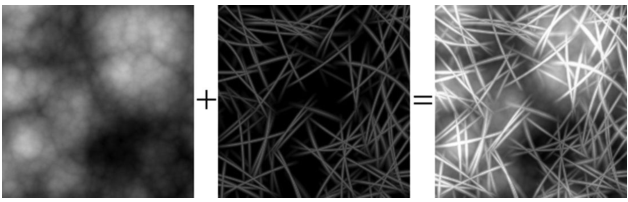
\includegraphics[width=\textwidth]{10-2}
    \centering
    \caption{源和目标颜色做加法。加法运算后,会创建更亮的图像。}
    \label{fig:10-2}
\end{figure}

\begin{flushleft}
我们可以使用上面的混合因子从目标像素中减去源像素,用 D3D12\_BLEND\_OP\_SUBTRACT 替换混合操作(图\ref{fig:10-3})。
\end{flushleft}

\begin{figure}[h]
    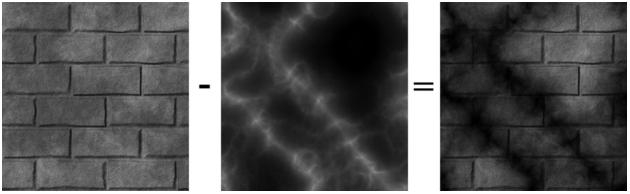
\includegraphics[width=\textwidth]{10-3}
    \centering
    \caption{从目标颜色中减去源颜色。由于颜色被移除,减法会产生较暗的图像。}
    \label{fig:10-3}
\end{figure}

%-------- 10.5.3 --------
\subsection{乘法(Multiplying)}
\begin{flushleft}
假设我们想要将源像素与其对应的目标像素相乘(参见图\ref{fig:10-4})。 为此,我们将源混合因子设置为 D3D12\_BLEND\_ZERO,将目标混合因子设置为D3D12\_BLEND\_SRC\_COLOR,将混合运算符设置为D3D12\_BLEND\_OP\_ADD。 通过此设置,混合等式可简化为:\\
\end{flushleft}

\begin{align*}
C&=C_{src}\otimes F_{src}\boxplus C_{dst}\otimes F_{dst}\\
C&=C_{src}\otimes (0,0,0)+C_{dst}\otimes C_{src}
C&=C_{dst}\otimes C_{src}
\end{align*}

\begin{figure}[h]
    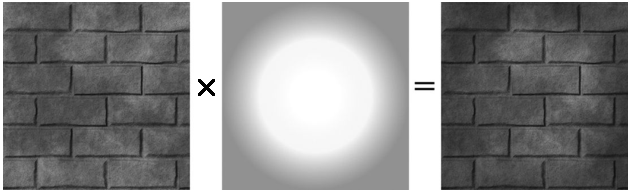
\includegraphics[width=\textwidth]{10-4}
    \centering
    \caption{源颜色与目标颜色相乘。}
    \label{fig:10-4}
\end{figure}

%-------- 10.5.4 --------
\subsection{透明度(Transparency)}
\begin{flushleft}
令源alpha分量被认为是控制源像素的不透明度的百分比(例如,0 alpha 表示 0%不透明,0.4表示40%不透明,1.0表示100%不透明)。 不透明度和透明度之间的关系只是$T=1-A$,其中$A$是不透明度,$T$是透明度。例如,如果某些东西是 0.4 不透明的,则它是 $1-0.4=0.6$透明。 现在假设我们想要根据源像素的不透明度混合源像素和目标像素。 要执行此操作,请将源混合因子设置为 D3D12\_BLEND\_SRC\_ALPHA,将目标混合因子设置为 D3D12\_BLEND\_INV\_SRC\_ALPHA,将混合运算符设置为 D3D12\_BLEND\_OP\_ADD。 通过此设置,混合等式可简化为:\\
\end{flushleft}

\begin{align*}
C&=C_{src}\otimes F_{src}\boxplus C_{dst}\otimes F_{dst}\\
C&=C_{src}\otimes (a_{s},a_{s},a_{s})+C_{dst}\otimes (1-a_{s},1-a_{s},1-a_{s})
C&=a_{s}C_{src}+(1-a_{s})C_{dst}
\end{align*}

\begin{flushleft}
例如,假设$s=0.25$,也就是说源像素仅为25%不透明。 然后当源像素和目标像素混合在一起时,我们期望最终颜色将是源像素的25%和目标像素的75%(源像素“后面”的像素)的组合,因为源像素是 75% 透明。上面的等式恰恰说明了这一点:\\
\end{flushleft}

\begin{align*}
C&=a_{s}C_{src}+(1-a_{s})C_{dst}
C&=0.25C_{src}+0.75C_{dst}
\end{align*}

\begin{flushleft}
使用这种混合方法,可以绘制透明对象,如图\ref{fig:10-1}中所示。 应该注意的是,使用这种混合方法,绘制对象的顺序很重要。我们使用以下规则:\\

绘制不使用混合的对象。按照与摄像机的距离对使用混合的对象进行排序,绘制以由后到前顺序使用混合的对象。\\

从后到前绘制顺序的原因是对象与空间背后的对象混合。 因为如果一个物体是透明的,我们可以通过它看到它背后的场景。 因此,必须将透明对象后面的所有像素都写入后缓冲区,以便我们可以将透明源像素与其后面场景的目标像素混合。\\

对于10.5.1中的混合方法,绘制顺序无关紧要,因为它只是阻止源像素写入后缓冲区。 对于10.5.2和10.5.3中讨论的混合方法,我们仍然首先绘制非混合对象,最后绘制混合对象; 这是因为我们希望在开始混合之前首先将所有非混合几何体放置在后缓冲区上。 但是,我们不需要对使用混合的对象进行排序。这是因为操作是可交换的。 也就是说,如果您从后缓冲区像素颜色B开始,然后对该像素执行$n$加法/减法/乘法混合,则顺序无关紧要:\\
\end{flushleft}

\begin{align*}
B^{'}&=B+C_{0}+C_{1}+...+C_{n-1}\\
B^{'}&=B-C_{0}-C_{1}-...-C_{n-1}\\
B^{'}&=B\otimes C_{0}\otimes C_{1}\otimes ...\otimes C_{n-1}
\end{align*}

%-------- 10.5.4 --------
\subsection{混合和深度缓冲(Blending and the Depth Buffer)}
\begin{flushleft}
当与加法/减法/乘法混合时,深度测试会出现问题。为了举例,我们将仅使用加法混合来解释,但是相同的想法适用于减法/乘法混合。如果我们使用加法混合渲染一组S对象,S中的对象不会相互模糊;相反,它们的颜色只是累积(见图\ref{fig:10-5})。因此,我们不希望在S中对象之间进行深度测试;因为如果我们这样做,没有从后到前的绘制顺序,S中的一个对象会遮挡S中的另一个对象,从而导致像素片段由于深度测试而被拒绝,这意味着对象的像素颜色不会被累积到混合总和中。可以通过在S中渲染对象时禁用对深度缓冲区的写入来禁用S中对象之间的深度测试。由于禁用了深度写入,因此使用加法混合绘制的S中对象的深度将不会写入深度缓冲区;因此,由于深度测试,该对象不会遮挡后面S中任何后来绘制的对象。请注意,我们仅在S中绘制对象时禁用深度写入(使用附加混合绘制的对象集)。深度读数和深度测试仍然启用。这样,非混合几何体(在混合几何体之前绘制)仍将模糊其后面的混合几何体。例如,如果在墙后面有一组加法混合的对象,则不会看到混合对象,因为实心墙遮挡了它们。如何禁用深度写入,配置深度测试设置将在下一章中介绍。
\end{flushleft}

\begin{figure}[h]
    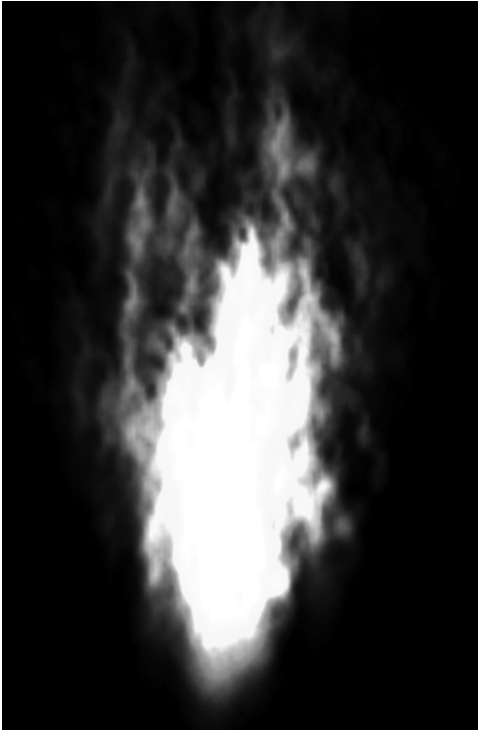
\includegraphics[width=\textwidth]{10-5}
    \centering
    \caption{通过加法混合,在更多颗粒重叠相加的源点附近强度更大。 随着颗粒扩散,强度减弱,因为较少的颗粒重叠相加。}
    \label{fig:10-5}
\end{figure}

\clearpage

%-------- 10.6 --------
\section{Alpha 通道(Alpha Channels)}
\begin{flushleft}
10.5.4节中的示例显示源alpha分量可用于RGB混合以控制透明度。 混合方程中使用的源颜色来自像素着色器。 正如我们在上一章中看到的,我们将漫反射材质的alpha值作为像素着色器的alpha输出返回。 因此,漫反射贴图的alpha通道用于控制透明度。\\
\end{flushleft}

\begin{align*}
float4 PS(VertexOut pin) : SV_Target
{
    float4 diffuseAlbedo = gDiffuseMap.Sample(
    gsamAnisotropicWrap, pin.TexC) * gDiffuseAlbedo;
    ...
    // Common convention to take alpha from diffuse albedo.
    litColor.a = diffuseAlbedo.a;
    return litColor;
}
\end{align*}

\begin{flushleft}
您通常可以在任何流行的图像编辑软件(如Adobe Photoshop)中添加Alpha通道,然后将图像保存为支持像DDS这样的Alpha通道的图像格式。\\
\end{flushleft}

%-------- 10.7 --------
\section{剪切像素(Clipping Pixels)}

\begin{flushleft}
有时我们希望完全拒绝进一步处理源像素。这可以通过内在的HLSL clip(x) 函数来完成。 此函数只能在像素着色器中调用,如果$x < 0$,它将丢弃当前像素进一步处理。此函数对于渲染线栅纹理很有用,例如,如图\ref{fig:10-6}所示。 也就是说,渲染像素的像素是完全不透明或完全透明的。
\end{flushleft}

\begin{figure}[h]
    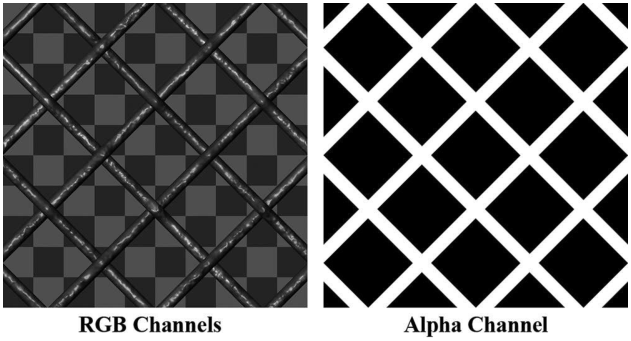
\includegraphics[width=\textwidth]{10-6}
    \centering
    \caption{alpha通道的铁丝网纹理。具有黑色alpha值的像素将被剪辑功能拒绝而不被绘制; 因此,只留下铁丝网。实质上,alpha通道用于从纹理中屏蔽非栅栏像素。}
    \label{fig:10-6}
\end{figure}

\begin{flushleft}
在像素着色器中,我们抓取纹理的alpha分量。 如果它是一个接近0的小值,表示该像素是完全透明的,那么将该像素剪辑做进一步处理。
\end{flushleft}

\begin{lstlisting}[escapechar=^]
float4 PS(VertexOut pin) : SV_Target
{
    float4 diffuseAlbedo = gDiffuseMap.Sample(
        gsamAnisotropicWrap, 
        pin.TexC) * gDiffuseAlbedo;

    ^\textbf{\#ifdef ALPHA\_TEST}^
    ^\textbf{// Discard pixel if texture alpha < 0.1. }^
    ^\textbf{// We do this test as soon }^
    ^\textbf{// as possible in the shader so that we can}^
    ^\textbf{// potentially exit the shader early, }^
    ^\textbf{// thereby skipping the rest of the shader code. }^
    ^\textbf{clip(diffuseAlbedo.a - 0.1f);}^
    ^\textbf{\#endif}^
    ...
    // Common convention to take alpha from diffuse albedo.
    litColor.a = diffuseAlbedo.a;
    return litColor;
}
\end{lstlisting}

\begin{flushleft}
观察只在定义了ALPHA\_TEST时剪辑; 这是因为我们可能不想为某些渲染项调用 clip ,因此需要能够通过使用专门的着色器来打开/关闭它。 此外,使用alpha测试需要付出代价,因此只应在需要时使用。\\

请注意,使用混合可以获得相同的结果,但这更有效。 首先,不需要进行混合计算(可以禁用混合)。 此外,绘制顺序无关紧要。 通过像素着色器早期丢弃像素,可以跳过剩余的像素着色器指令(对丢弃的像素进行计算没有意义)。\\
~\\
NOTICE: 受到滤镜影响,alpha通道可能会有点模糊,因此在剪切像素时应留下一些缓冲空间。 例如,剪切像素的alpha值接近0,但不一定恰好为零。
~\\

图\ref{fig:10-7}显示了“Blend”演示的屏幕截图。 它使用透明混合渲染半透明水,并使用剪辑测试渲染线栅栏箱。 值得一提的另一个变化是,可以通过带有栅栏纹理的箱子看到,禁用alpha测试的背面剔除对象:\\
\end{flushleft}

\begin{lstlisting}
// PSO for alpha tested objects
D3D12_GRAPHICS_PIPELINE_STATE_DESC alphaTestedPsoDesc
    = opaquePsoDesc;
alphaTestedPsoDesc.PS =
{
    reinterpret_cast<BYTE*>(
        mShaders[“alphaTestedPS”]->GetBufferPointer()),
        mShaders[“alphaTestedPS”]->GetBufferSize()
};
alphaTestedPsoDesc.RasterizerState.CullMode =
    D3D12_CULL_MODE_NONE;
ThrowIfFailed(
    md3dDevice->CreateGraphicsPipelineState(
        &alphaTestedPsoDesc,
        IID_PPV_ARGS(&mPSOs[“alphaTested”])));
\end{lstlisting}

\begin{figure}[h]
    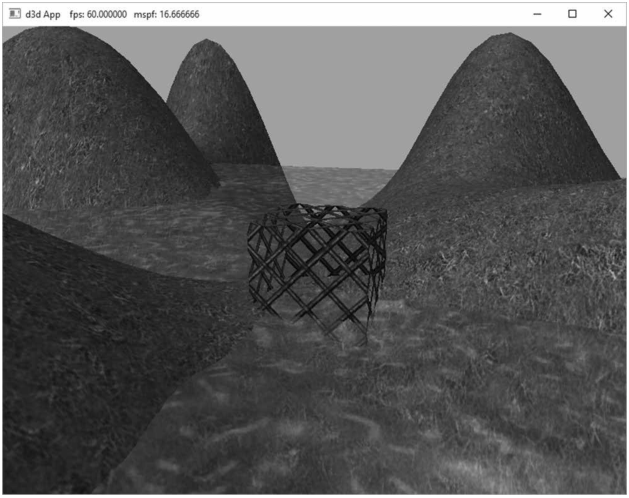
\includegraphics[width=\textwidth]{10-7}
    \centering
    \caption{“混合”演示截图。}
    \label{fig:10-7}
\end{figure}

%-------- 10.8 --------
\section{雾(FOG)}
\begin{flushleft}
为了模拟游戏中的某些类型的天气条件,我们需要能够实现雾效果; 见图\ref{fig:10-8}。 雾提供一些附带的好处。例如,它可以屏蔽远程渲染物体并防止弹出。 弹出是指由于摄像机的移动,之前在远处平面后面的物体突然出现在平截头体前面,因此变得可见; 在远处设置一层雾,能让弹出变得隐蔽。 请注意,如果场景在晴朗的日子进行,可能希望在远距离处仍然包含微量的雾模拟这种大气透视现象,因为即使在晴朗的日子,远处的物体(如山脉)也会变得朦胧,并且会因深度而失去对比度。\\
\end{flushleft}

\begin{figure}[h]
    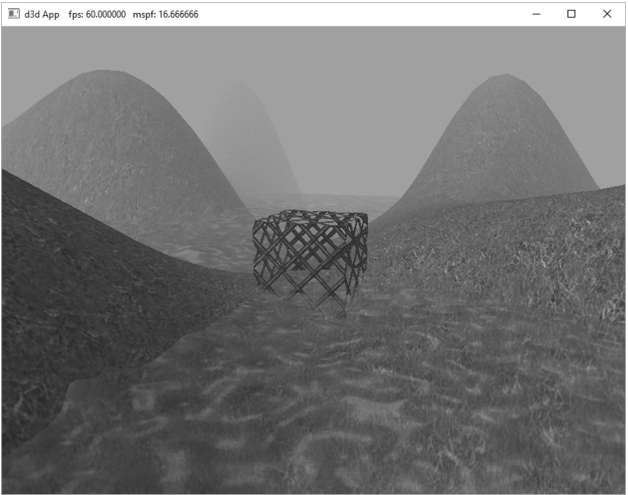
\includegraphics[width=\textwidth]{10-8}
    \centering
    \caption{启用雾的“混合”演示截图。}
    \label{fig:10-8}
\end{figure}

\begin{figure}[h]
    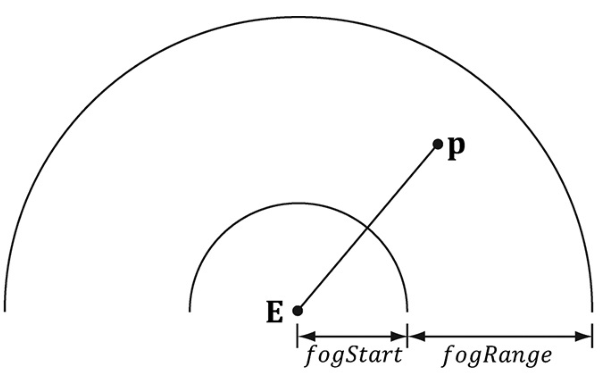
\includegraphics[width=\textwidth]{10-9}
    \centering
    \caption{距离视点的距离,以及fogStart和fogRange参数。}
    \label{fig:10-9}
\end{figure}

\begin{flushleft}
实施雾的策略如下:指定雾颜色,相机的雾起始距离和雾范围(即从雾开始距离到雾完全隐藏任何物体的范围)。然后三角形上的点的颜色是其通常颜色和雾颜色的加权平均值:\\
\end{flushleft}

\begin{align*}
foggedColor&=litColor+s(fogColor-litColor)
&=(1-s)\cdot litColor+s\cdot fotColor
\end{align*}

\begin{flushleft}
参数s的范围是0到1,它是摄像机位置和表面点之间距离的函数。 随着表面点和眼睛之间的距离增加,该点变得越来越模糊。 参数s定义如下:\\
\end{flushleft}

\begin{align*}
s=saturate\left ( \frac{dist(\boldsymbol{p},\boldsymbol{E})-fotStart}{fogRange}\right )
\end{align*}

\begin{flushleft}
其中 $dist(\boldsymbol{p},\boldsymbol{E})$是表面点$\boldsymbol{p}$和摄像机位置$\boldsymbol{E}$之间的距离。saturate 函数将参数钳位到范围$[0,1]$:\\
\end{flushleft}

\begin{align*}
saturate(x)=\left\{\begin{matrix}
x,0\leq x\leq 1\\ 
0,x<0\\ 
1,x>1
\end{matrix}\right.
\end{align*}

\begin{flushleft}
图\ref{fig:10-10}显示了$s$作为距离函数的图。我们看到当$dist(\boldsymbol{p},\boldsymbol{E})\leq pogstStart$时,$s=0$并且雾化的颜色由下式给出:\\
\end{flushleft}

\begin{align*}
foggedColor=litColor
\end{align*}

\begin{figure}[h]
    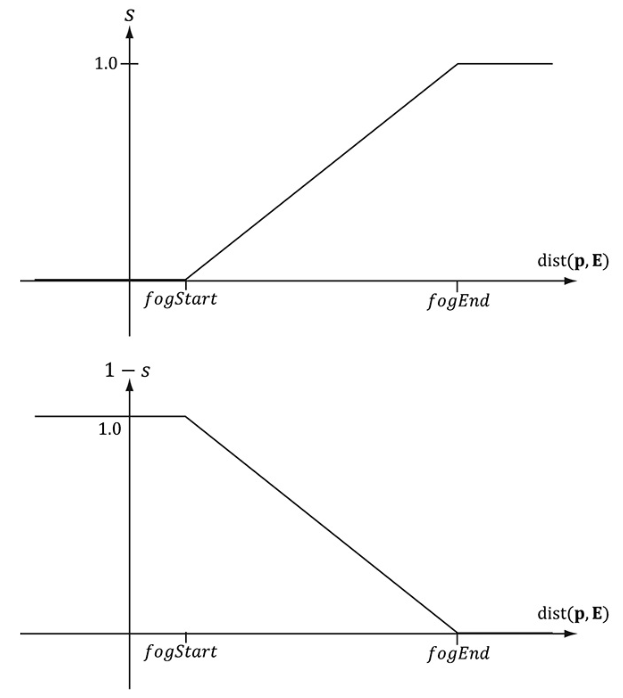
\includegraphics[width=\textwidth]{10-10}
    \centering
    \caption{(上):作为距离函数的$s$(雾色权重)图。(下):$1-s$(亮色权重)作为距离函数的图。 随着$s$增加,$(1-s)$减少相同的量。}
    \label{fig:10-10}
\end{figure}

\begin{flushleft}
换句话说,雾不会修改与相机的距离小于$fogStart$的顶点的颜色。 在距离相机的距离至少为$fogStart$的距离之前,雾不会开始影响颜色。\\

设$fogEnd=fogStart$,当 $dist(\boldsymbol{p},\boldsymbol{E})\geq fogEnd$时,$s=1$,且被雾影响的颜色为 $foggedColor=fogColor$\\

也就是说,雾完全隐藏在大于或等于$fogEnd$的距离处的表面点——所以你看到的就是雾的颜色。\\

当$fogStart<dist(\boldsymbol{p},\boldsymbol{E})<fogEnd$时,我们看到当$dist(\boldsymbol{p},\boldsymbol{E})$从$fogStart$增加到$fogEnd$时,$s$线性地从$0$上升到$1$。 这意味着随着距离的增加,雾的颜色变得越来越重,而原始颜色的权重越来越少。 因为随着距离的增加,雾会越来越使表面点变得模糊。\\

以下着色器代码显示了雾的实现方式。在计算出亮色后,计算像素级别的距离和插值。\\
\end{flushleft}

\begin{lstlisting}[escapechar=^]
//*********************************************************
// Default.hlsl by Frank Luna (C) 2015 All Rights Reserved.
//
// Default shader, currently supports lighting.
//*********************************************************

// Defaults for number of lights.
#ifndef NUM_DIR_LIGHTS
    #define NUM_DIR_LIGHTS 3
#endif

#ifndef NUM_POINT_LIGHTS
    #define NUM_POINT_LIGHTS 0
#endif

#ifndef NUM_SPOT_LIGHTS
    #define NUM_SPOT_LIGHTS 0
#endif

// Include structures and functions for lighting.
#include "LightingUtil.hlsl"

Texture2D    gDiffuseMap : register(t0);


SamplerState gsamPointWrap        : register(s0);
SamplerState gsamPointClamp       : register(s1);
SamplerState gsamLinearWrap       : register(s2);
SamplerState gsamLinearClamp      : register(s3);
SamplerState gsamAnisotropicWrap  : register(s4);
SamplerState gsamAnisotropicClamp : register(s5);

// Constant data that varies per frame.
cbuffer cbPerObject : register(b0)
{
    float4x4 gWorld;
    float4x4 gTexTransform;
};

// Constant data that varies per pass.
cbuffer cbPass : register(b1)
{
    float4x4 gView;
    float4x4 gInvView;
    float4x4 gProj;
    float4x4 gInvProj;
    float4x4 gViewProj;
    float4x4 gInvViewProj;
    float3 gEyePosW;
    float cbPerObjectPad1;
    float2 gRenderTargetSize;
    float2 gInvRenderTargetSize;
    float gNearZ;
    float gFarZ;
    float gTotalTime;
    float gDeltaTime;
    float4 gAmbientLight;

    ^\textbf{// Allow application to change fog parameters once per frame.}^
    ^\textbf{// For example, we may only use fog for certain times of day.}^
    ^\textbf{float4 gFogColor;}^
    ^\textbf{float gFogStart;}^
    ^\textbf{float gFogRange;}^
    float2 cbPerObjectPad2;

    // Indices [0, NUM_DIR_LIGHTS) are directional lights;
    // indices [NUM_DIR_LIGHTS, NUM_DIR_LIGHTS+NUM_POINT_LIGHTS) 
                are point lights;
    // indices [NUM_DIR_LIGHTS+NUM_POINT_LIGHTS, 
    //         NUM_DIR_LIGHTS+NUM_POINT_LIGHT+NUM_SPOT_LIGHTS)
    // are spot lights for a maximum of MaxLights per object.
    Light gLights[MaxLights];
};

cbuffer cbMaterial : register(b2)
{
    float4   gDiffuseAlbedo;
    float3   gFresnelR0;
    float    gRoughness;
    float4x4 gMatTransform;
};

struct VertexIn
{
    float3 PosL    : POSITION;
    float3 NormalL : NORMAL;
    float2 TexC    : TEXCOORD;
};

struct VertexOut
{
    float4 PosH    : SV_POSITION;
    float3 PosW    : POSITION;
    float3 NormalW : NORMAL;
    float2 TexC    : TEXCOORD;
};

VertexOut VS(VertexIn vin)
{
    VertexOut vout = (VertexOut)0.0f;
    
    // Transform to world space.
    float4 posW = mul(float4(vin.PosL, 1.0f), gWorld);
    vout.PosW = posW.xyz;

    // Assumes nonuniform scaling; otherwise, need to use inverse-transpose of world matrix.
    vout.NormalW = mul(vin.NormalL, (float3x3)gWorld);

    // Transform to homogeneous clip space.
    vout.PosH = mul(posW, gViewProj);
    
    // Output vertex attributes for interpolation across triangle.
    float4 texC = mul(float4(vin.TexC, 0.0f, 1.0f), gTexTransform);
    vout.TexC = mul(texC, gMatTransform).xy;

    return vout;
}

float4 PS(VertexOut pin) : SV_Target
{
    float4 diffuseAlbedo = gDiffuseMap.Sample(gsamAnisotropicWrap, pin.TexC) * gDiffuseAlbedo;
    
#ifdef ALPHA_TEST
    // Discard pixel if texture alpha < 0.1.  We do this test as soon 
    // as possible in the shader so that we can potentially exit the
    // shader early, thereby skipping the rest of the shader code.
    clip(diffuseAlbedo.a - 0.1f);
#endif

    // Interpolating normal can unnormalize it, so renormalize it.
    pin.NormalW = normalize(pin.NormalW);

    // Vector from point being lit to eye. 
    float3 toEyeW = gEyePosW - pin.PosW;
    float distToEye = length(toEyeW);
    toEyeW /= distToEye; // normalize

    // Light terms.
    float4 ambient = gAmbientLight*diffuseAlbedo;

    const float shininess = 1.0f - gRoughness;
    Material mat = { diffuseAlbedo, gFresnelR0, shininess };
    float3 shadowFactor = 1.0f;
    float4 directLight = ComputeLighting(gLights, mat, pin.PosW,
        pin.NormalW, toEyeW, shadowFactor);

    float4 litColor = ambient + directLight;

^\textbf{\#ifdef FOG}^
    ^\textbf{float fogAmount = saturate((distToEye - gFogStart) / gFogRange);}^
    ^\textbf{litColor = lerp(litColor, gFogColor, fogAmount);}^
^\textbf{\#endif}^

    // Common convention to take alpha from diffuse albedo.
    litColor.a = diffuseAlbedo.a;

    return litColor;
}
\end{lstlisting}

\begin{flushleft}
有些场景可能不想使用雾; 因此,我们通过在编译着色器时要求定义FOG来使雾成为可选的。 这样,如果不想要雾,那么我们不支付雾计算的成本。 在演示中,通过向 CompileShader 函数提供以下 D3D\_SHADER\_MACRO 来启用雾:\\
\end{flushleft}

\begin{lstlisting}
const D3D_SHADER_MACRO defines[] =
{
    "FOG", "1",
    NULL, NULL
};
mShaders["opaquePS"] = d3dUtil::CompileShader(
    L"Shaders\Default.hlsl", 
    defines, 
    "PS", 
    "ps_5_0");
\end{lstlisting}

\begin{flushleft}
~\\
NOTICE: 观察在雾计算中,会使用$distToEye$值,和计算标准化$toEye$向量。 一个不太理想的实现就是:\\
\end{flushleft}

\begin{lstlisting}
float3 toEye = normalize(gEyePosW - pin.PosW);
float distToEye = distance(gEyePosW, pin.PosW);
\end{lstlisting}

\begin{flushleft}
这基本上计算了两次$toEye$向量的长度,一次是在$normalize$函数中,一次是在$distance$函数中。
~\\
\end{flushleft}

%-------- 10.9 --------
\section{总结}
\begin{flushleft}
1.混合是一种技术,它允许我们将当前光栅化的像素(所谓的源像素)与先前光栅化到后缓冲区的像素(所谓的目标像素)混合(组合)。 这种技术使我们能够渲染半透明物体,如水和玻璃。\\

2.混合公式:\\
\end{flushleft}
\begin{align*}
C&=C_{src}\otimes F_{src}\boxplus C_{dst}\otimes F_{dst}\\
A&=A_{src}F_{src}\boxplus A_{dst}F_{dst}
\end{align*}
\begin{flushleft}
注意 RGB 分量与 alpha 分量相互独立。二元运算符$\boxplus$由枚举类 D3D12\_BLEND\_OP 定义。\\

3.$F_{src}$,$F_{dst}$,$F_{src}$和$F_{dst}$称为混合因子,它们提供了一种自定义混合方程的方法。它们是 D3D12\_BLEND 枚举类型的成员。 对于alpha混合等式,不允许以\_COLOR结尾的混合因子。\\

4.源alpha信息来自漫反射材质。 在我们的框架中,漫反射材质由纹理贴图定义,纹理的alpha通道存储alpha信息。\\

5.使用内部HLSL clip(x) 函数可以完全拒绝源像素进一步处理。 此功能只能在像素着色器中调用,如果$x<0$,在当前像素进一步处理时它会被丢弃。除此之外,当像素是完全不透明或完全透明的(它用于拒绝完全透明的像素——像素值接近零的像素)时,此函数可用于提高渲染像素的效率。\\

6.使用雾来模拟各种天气效果和大气透视,隐藏远处的渲染瑕疵,隐藏弹出。 在我们的线性雾模型中,指定雾颜色,相机的雾起始距离和雾范围。 三角形上的点的颜色是其通常颜色和雾颜色的加权平均值:\\
\end{flushleft}

\begin{align*}
foggedColor&=litColor+s(fogColor-litColor)\\
&=(1-s)\cdot litColor+s\cdot fogColor
\end{align*}

\begin{flushleft}
参数$s$的范围是$0$到$1$,它是摄像机位置和表面点之间距离的函数。 随着表面点和眼睛之间的距离增加,该点变得越来越模糊。
\end{flushleft}

%-------- 10.10 --------
\section{练习}
\begin{flushleft}
1.尝试不同的混合操作和混合因子组合。\\
2.修改"混合"演示,从绘制水开始。解释结果。\\
3.假设$fogStart=10$且$fogRange=200$。根据如下情况计算 $foggedColor$值。\\
\begin{itemize}
  \item a.$dist(\boldsymbol{p},\boldsymbol{E})$=160
  \item b.$dist(\boldsymbol{p},\boldsymbol{E})$=110
  \item c.$dist(\boldsymbol{p},\boldsymbol{E})$=60
  \item d.$dist(\boldsymbol{p},\boldsymbol{E})$=30
\end{itemize}
4.查看生成的着色器程序汇编代码,验证未定义 ALPHA\_TEST 的编译像素着色器没有 discard 指令,然后再定义 ALPHA\_TEST 编译像素着色器,观察区别。discard 指令对应于 HLSL 的 clip 指令。\\

5.修改"混合"演示,创建和应用混合渲染状态,使该状态禁用对红色和绿色通道的颜色写入。\\
\end{flushleft}


